\section{Deployment}

% Explain here how to install and launch the produced software artefacts.
% %
% Assume the softaware must be installed on a totally virgin environment.
% %
% So, report \textbf{any} configuration step.

% Gradle and Docker may be useful here to ensure the deployment and launch processes to be easy.

Per eseguire il deploy dell'applicazione abbiamo scelto di utilizzare Docker, nello specifico, l'architettura viene servita attraverso i seguenti container:

\begin{itemize}
    \item \textbf{Frontend Service}: Container che serve il Frontend sotto forma di Single Page Application.

    \item \textbf{Messages Service e relativo Db}: Microservizio responsabile della gestione dei messaggi testuali dell'applicazione (invio, ricezione, ecc...).

    \item \textbf{Monitoring Service e relativo Db}: Microservizio responsabile del monitoraggio dello stato di tutti i microservizi.

    \item \textbf{Notifications Service e relativo Db}: Mircoservizio responsabile delle notifiche degli utenti. Inoltre, detiene l'online status degli utenti del sistema.

    \item \textbf{Piperchat Service e relativo Db}: Microservizio responsabile della gestione dei Server e dei Canali dell'applicazione (creazione, modifica, partecipanti, ecc...).

    \item \textbf{Users Service e relativo Db}: Microservizio responsabile della gestione degli utenti dell'applicazione (login, registrazione, amicizie, ecc...).

    \item \textbf{Multimedia Service e relativo Db}: Microservizio responsabile della gestione delle chiamate infra-utenti e dei canali multimediali.

    \item \textbf{Broker}: Container che ospita un server di \emph{RabbitMQ} per permettere lo scambio di messaggi all'interno del sistema

    \item \textbf{Coturn}: Container che ospita il server \emph{TURN} (\url{https://github.com/coturn/coturn})

    \item \textbf{Gateway}: Container che ospita l'\emph{API Gateway} realizzato con \emph{Traefik}. 

    \item \textbf{Inspector}: Container di \emph{utility} per debuggare e/o ispezionare i servizi dall'interno della rete.
\end{itemize}

Per ogni microservizio quindi, viene effettuato il deploy di due diversi container, uno per il Webserver, mentre l'altro per il relativo database non relazionale.

Ogni microservizio possiede le seguenti reti docker:

\begin{itemize}
    \item \textbf{Frontend}: Rete necessaria per ricevere le richieste dal frontend tramite il Gateway.

    \item \textbf{Backend}: Rete necessaria per comunicare internamente con gli altri microservizi (nel nostro caso tramite message broker).

    \item \textbf{Microservicename-network}: Rete interna del microservizio, utile alla comunicazione con il proprio database.
\end{itemize}

%
%
%
\subsection{Build dell'immagine Docker di PiperChat}

Si è deciso di realizzare un'immagine Docker unica per l'intero progetto.
%
Per eseguire successivamente i vari servizi è possibile utilizzare tale immagine e modificare opportunamente il comando iniziale.

Di seguito è riportato un esempio per utilizzare l'immagine di \texttt{piperchat}:

\begin{verbatim}
docker build . --tag piperchat
docker run piperchat npm run --workspace ./services/users start
\end{verbatim}

%
%
%
\subsection{Deploy singolo Microservizio}

Per il deploy di ogni singolo microservizio è stato scritto un file di \texttt{Docker Compose}.
%
Esso predispone l'ambiente necessario al container (reti, labels, volumi, etc.) per essere eseguito correttamente.
%
Successivamente viene utilizzata l'immagine precedentemente creata, con il comando sovrascritto opportunamente per lo specifico microservizio.

Esempio di Docker compose relativo al singolo microservizio:

\begin{lstlisting}[style=yaml, caption={microservice Test}, label=lst:compose-yaml]
services:
  piperchat-service:
    image: piperchat
    command: [
        'npm', 
        'run', 
        '--workspace', 
        './services/piperchat', 
        'start'
    ]
    expose:
      - '${PIPERCHAT_SERVICE_PORT}'
    depends_on:
      db-piperchat-service:
        condition: service_healthy
      broker:
        condition: service_healthy
    networks:
      piperchat-network:
      backend:
        aliases:
          - ${PIPERCHAT_SERVICE_NAME}
      frontend:
    environment:
      - PORT=${PIPERCHAT_SERVICE_PORT}
      - AMQP_URI=${BROKER_URI}
      - MONGO_URI=
        mongodb://db-piperchat-service:27017/piperchat
    labels:
      - |
        traefik.http.routers.piperchat-service.rule=
        (Method(`GET`, `POST`) && Path(`/servers`)) ||
            ... other paths

  db-piperchat-service:
    image: mongo
    expose:
      - '27017'
    volumes:
      - './.docker/db-piperchat:/data/db'
    healthcheck:
      test: |
        host=`hostname --ip-address || echo '127.0.0.1'`;
        mongo --quiet $${host}/test --eval 
        'quit(db.runCommand({ ping: 1 }).ok ? 0 : 2)' 
        && echo 0 || echo 1
    networks:
      - piperchat-network

networks:
  piperchat-network:

\end{lstlisting}

%
%
%
\subsection{Deploy dell'architettura}

Come accennato in precedenza, per ogni microservizio è stato scritto un apposito file di \texttt{Docker Compose}.
%
L'unione di tutti i \texttt{docker-compose.yaml} è stata automatizzata tramite uno script bash, che permette di operare sull'intera architettura, aggregando precedentemente i file di tutti i microservizi.
%
Lo script é \href{https://github.com/zucchero-sintattico/piperchat/blob/develop/composeAll.sh}{\texttt{./composeAll.sh}}.

Di seguito è riportata l'intera architettura di cui viene eseguito il deploy, con tutti i microservizi, i relativi database, le reti, il broker ed il gateway.

% \begin{verbatim}
% #!/bin/bash
% docker compose \
%     --project-name piperchat \
%     --project-directory . \
%     --env-file ./.env \
%     -f ./services/broker/docker-compose.yaml \
%     -f ./services/frontend/docker-compose.yaml \
%     -f ./services/gateway/docker-compose.yaml \
%     -f ./services/messages/docker-compose.yaml \
%     -f ./services/monitoring/docker-compose.yaml \
%     -f ./services/notifications/docker-compose.yaml \
%     -f ./services/piperchat/docker-compose.yaml \
%     -f ./services/users/docker-compose.yaml \
%     -f ./services/multimedia/docker-compose.yaml \
%     -f ./dev/inspector.docker-compose.yaml \
%     $@
% \end{verbatim}

\begin{figure}[H]
    \centering
    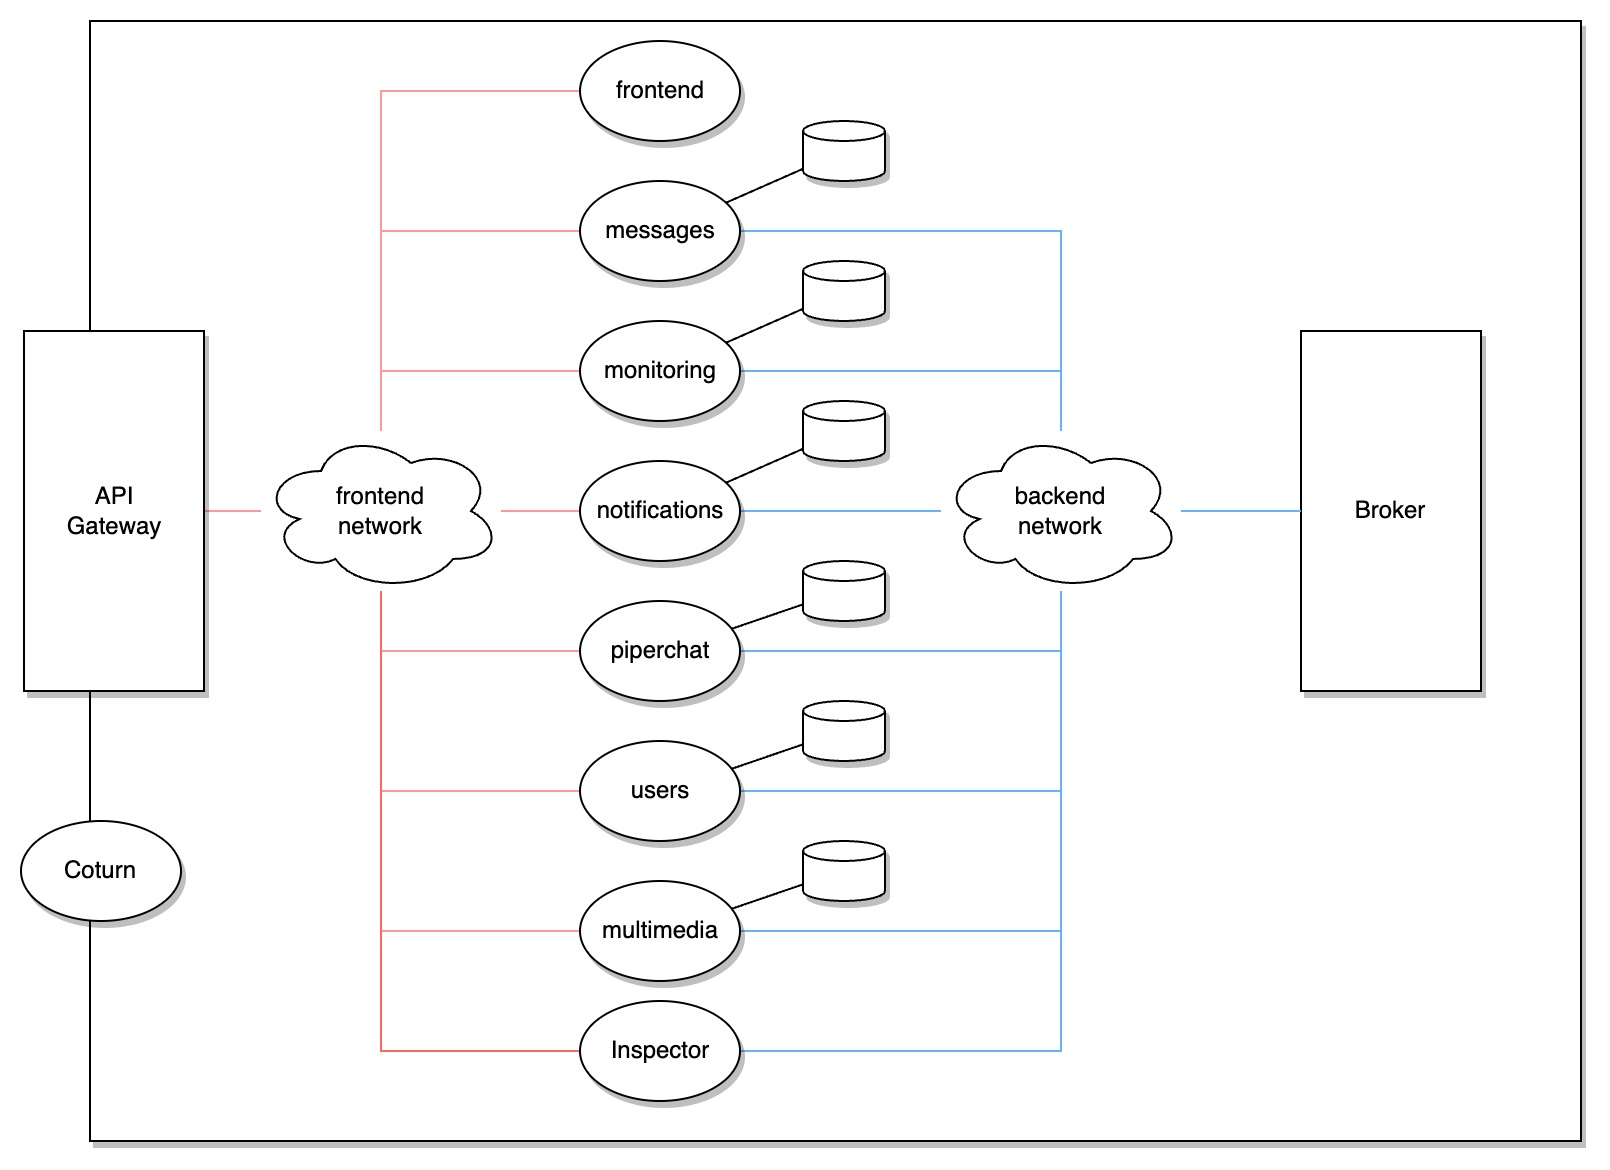
\includegraphics[width=\textwidth]{sections/06-deployment/img/microservice-deployment.jpg}
    \label{fig:architecture-deployment}
    % \caption{Deploy dei vari container e le relative reti.}
\end{figure}

%
%
%
\subsection{Testing deploy}

Per effettuare il testing lato Backend, è stato realizzato un ulteriore \texttt{Docker Compose} il quale ci ha permesso deployare un infrastruttura “alleggerita", dotata unicamente dei container necessari a testare i singoli microservizi, nonché:

\begin{itemize}
    \item Un'istanza del Broker

    \item Un'istanza del database

    \item Un'istanza di Mongo Express per visualizzare il database
\end{itemize}

Questo \texttt{Docker Compose} è situato nella cartella \texttt{/dev}, insieme allo script che ne automatizza l'esecuzione, chiamato \texttt{runDev.sh}.

Di seguito riportato il \texttt{Docker Compose} dell'infrastruttura usata per il testing:

\begin{lstlisting}[style=yaml, caption={Testing Deploy}, label=lst:testing:deploy]
services:
  db-service:
    image: mongo
    ports:
      - '27017:27017'
    healthcheck:
      test: |
        host=`hostname --ip-address || echo '127.0.0.1'`;
        mongo --quiet $${host}/test --eval
            'quit(db.runCommand({ ping: 1 }).ok ? 0 : 2)' 
            && echo 0 || echo 1

  broker:
    image: rabbitmq:3-management-alpine
    ports:
      - '5672:5672'
      - '15672:15672'
    healthcheck:
      test: ['CMD', 'rabbitmq-diagnostics', '-q', 'ping']

  mongo-express:
    image: mongo-express:latest
    restart: always
    ports:
      - '8081:8081'
    environment:
      ME_CONFIG_MONGODB_SERVER: 'db-service'
    depends_on:
      db-service:
        condition: service_healthy

\end{lstlisting}

%
%
%
\subsection{Istruzioni per il Deployment}

Di seguito, elencate le istruzioni per eseguire il deploy dell'applicazione:

\begin{enumerate}
    \item Clone del Repository:
\begin{verbatim}
$ git clone https://github.com/zucchero-sintattico/piperchat.git
\end{verbatim}

    \item Installazione delle dipendenze:
\begin{verbatim}
$ npm i
\end{verbatim}

    \item Copia del file contenente le variabili di environment dal template:
\begin{verbatim}
$ cp .env.template .env
\end{verbatim}

    \item Eseguire il deploy dell'architettura tramite lo script che esegue anche il build dell'immagine:
\begin{verbatim}
$ ./cleanDeploy.sh
\end{verbatim}

    \item Dalla seconda volta in poi, per rieseguire il deploy dell'architettura mantenendo i volumi e le immagini precedentemente create, basterà lanciare lo script:
\begin{verbatim}
$ ./deploy.sh
\end{verbatim}
\end{enumerate}
